\section*{Acknowledgments}
We acknowledge the support of T\"UB\.{I}TAK (the Scientific and Technological Research Council of T\"urkiye)
projects 124E091 and 124N941. The authors used Claude to enhance the
manuscript by shortening sentences, correcting typos, and improving grammar.

\bibliographystyle{IEEEtran}
\bibliography{refs}

% IEEE biographies belong to the journal submission.
\ifsubmission
\begin{IEEEbiography}
[{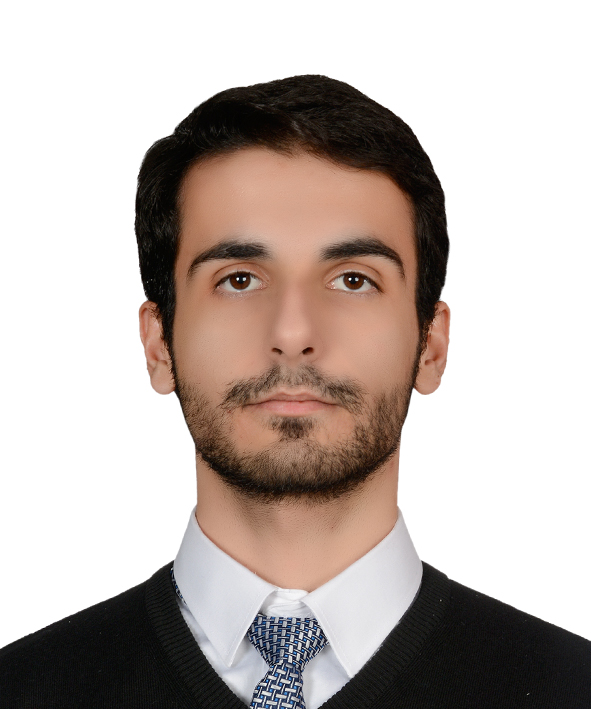
\includegraphics[width=1in,height=1.25in,clip,keepaspectratio]{authors/hkanpak.jpg}}]
{HALİL İBRAHİM KANPAK}~received his B.Sc. degree in Mathematics from Koç University. He is currently pursuing his Ph.D. at Koç University, where he is a member of the Cryptography, Cyber Security \& Privacy Research Group. His research interests include cryptography and related areas in Deep Learning.
\end{IEEEbiography}

\begin{IEEEbiography}
[{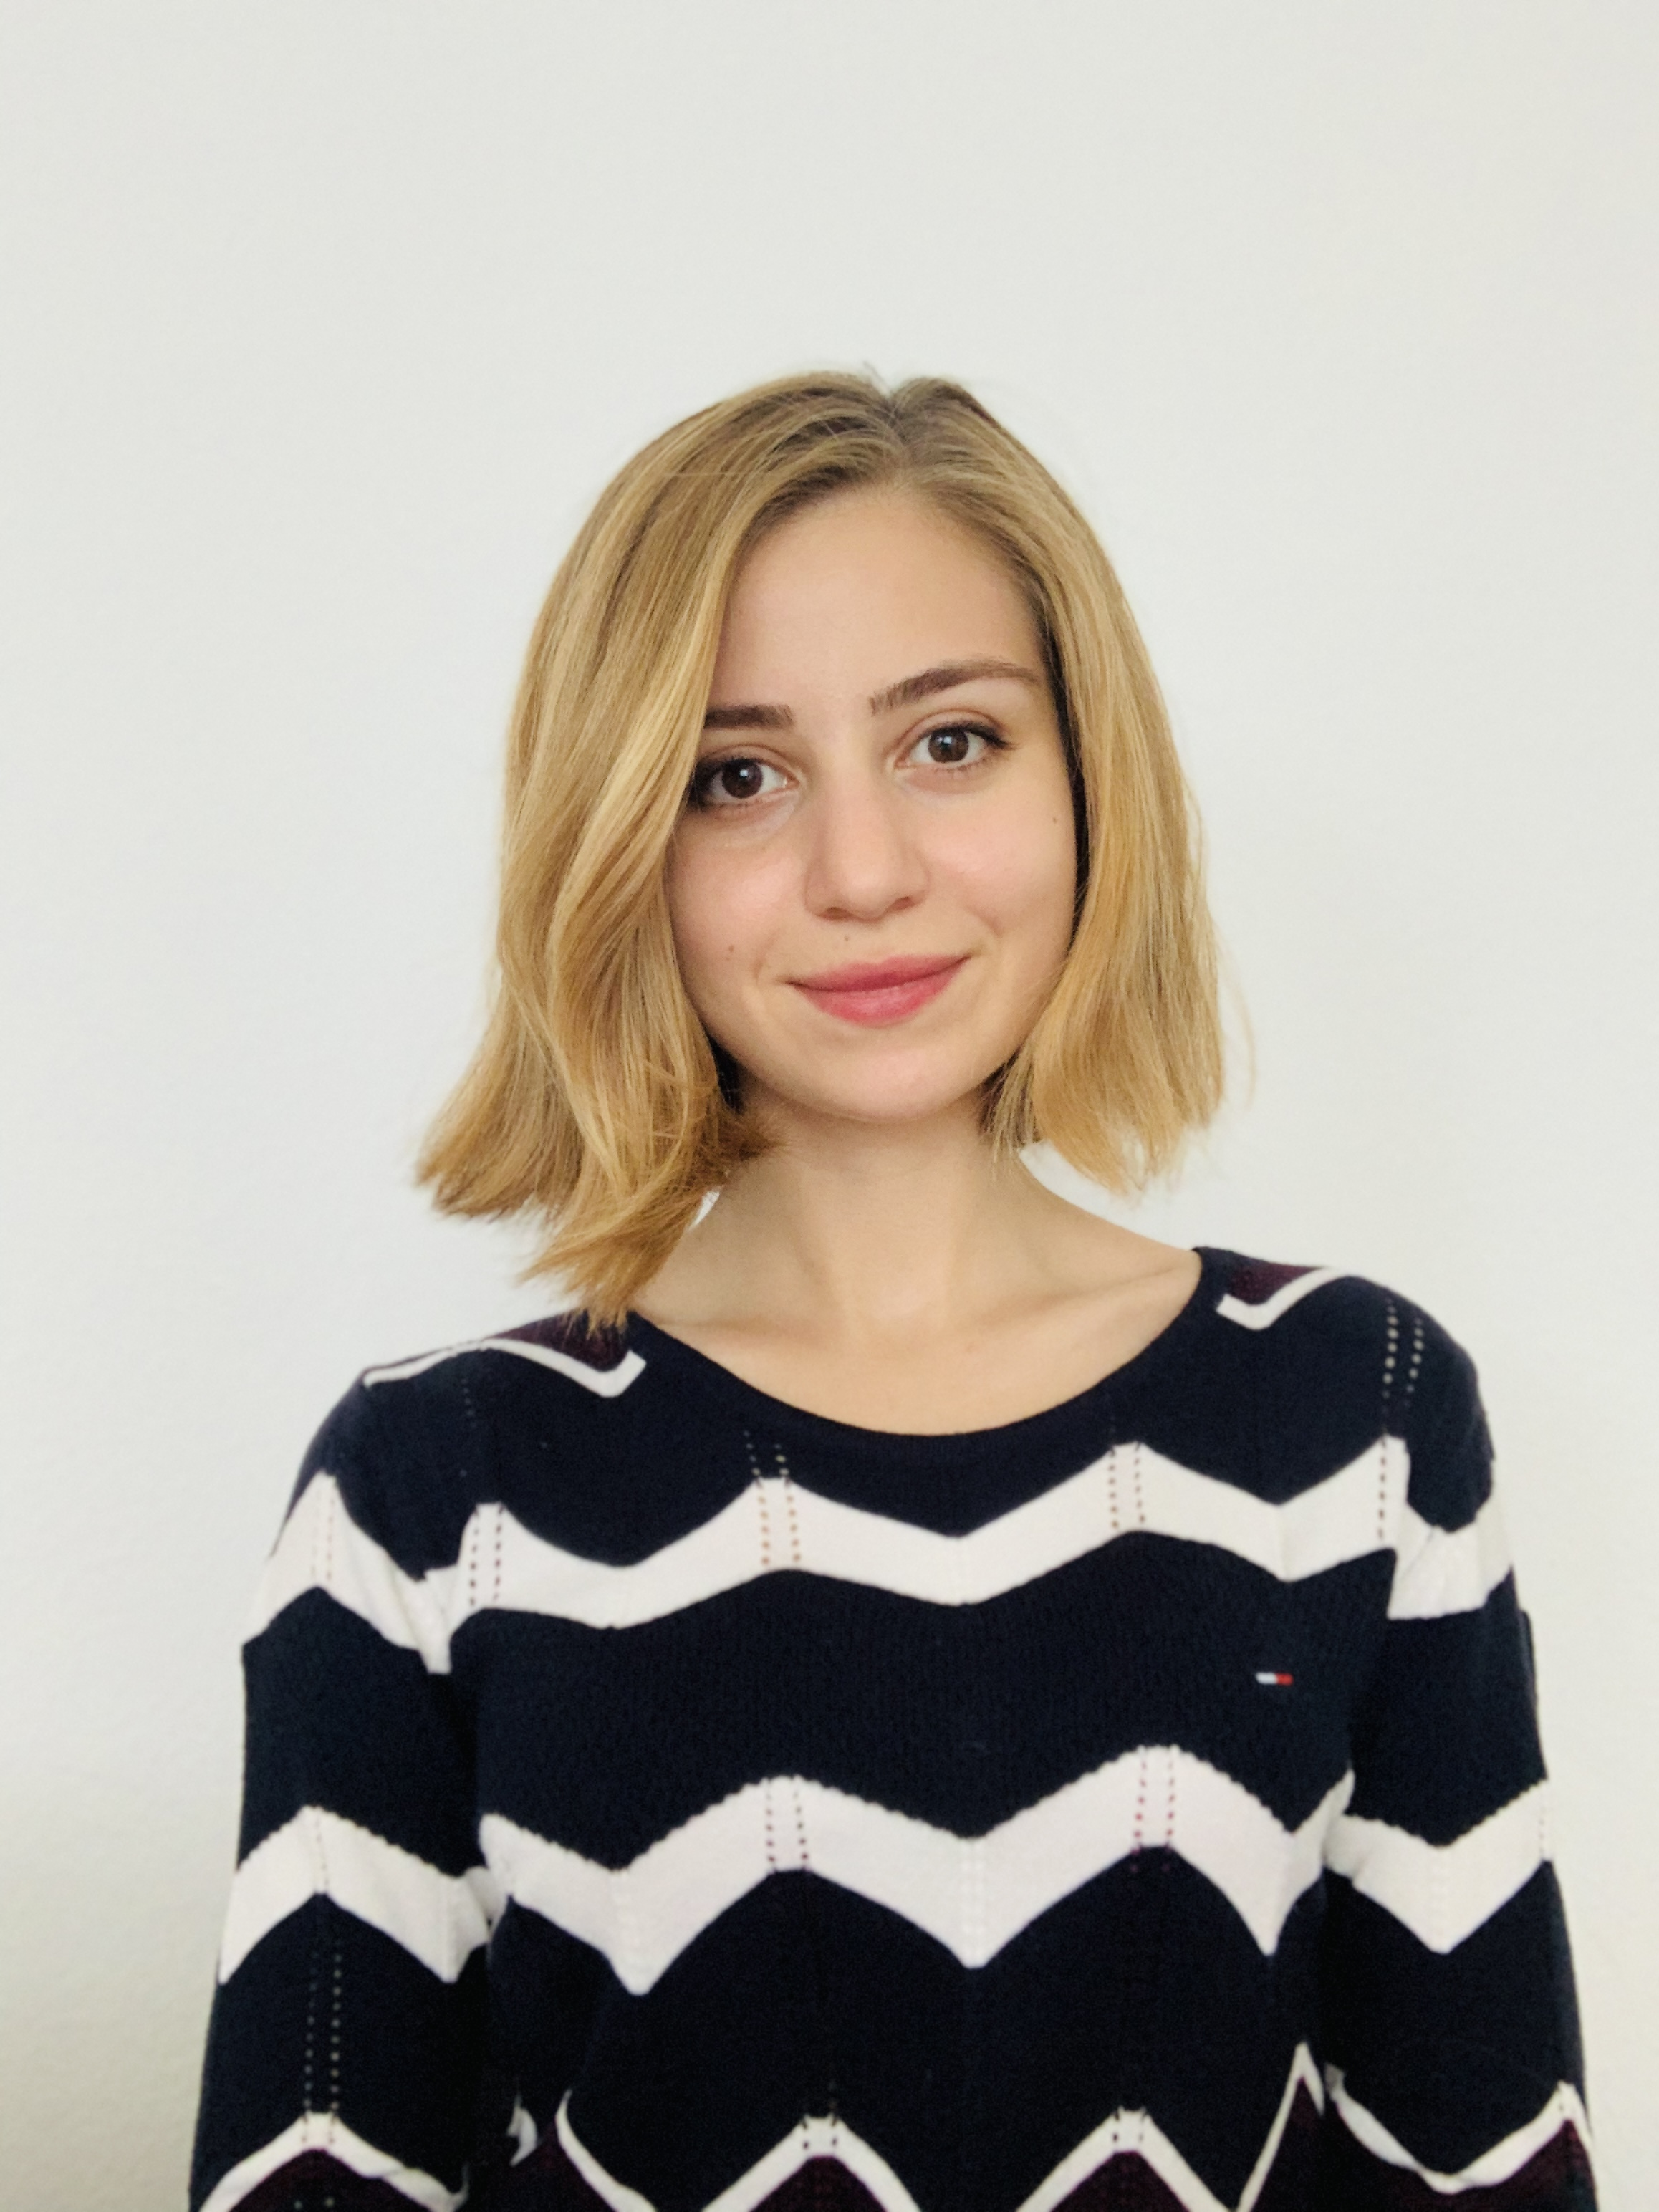
\includegraphics[width=1in,height=1.25in,clip,keepaspectratio]{authors/sinem.jpg}}]
{Asst. Prof. SİNEM SAV}~received her Ph.D. in Computer and Communication Sciences from École Polytechnique Fédérale de Lausanne (EPFL). She also holds M.Sc. and B.Sc. degrees in Computer Engineering from Bilkent University, where she currently serves as an Assistant Professor in the Computer Engineering department. Her research interests include privacy-preserving machine learning and applied cryptography.
\end{IEEEbiography}

\begin{IEEEbiography}
[{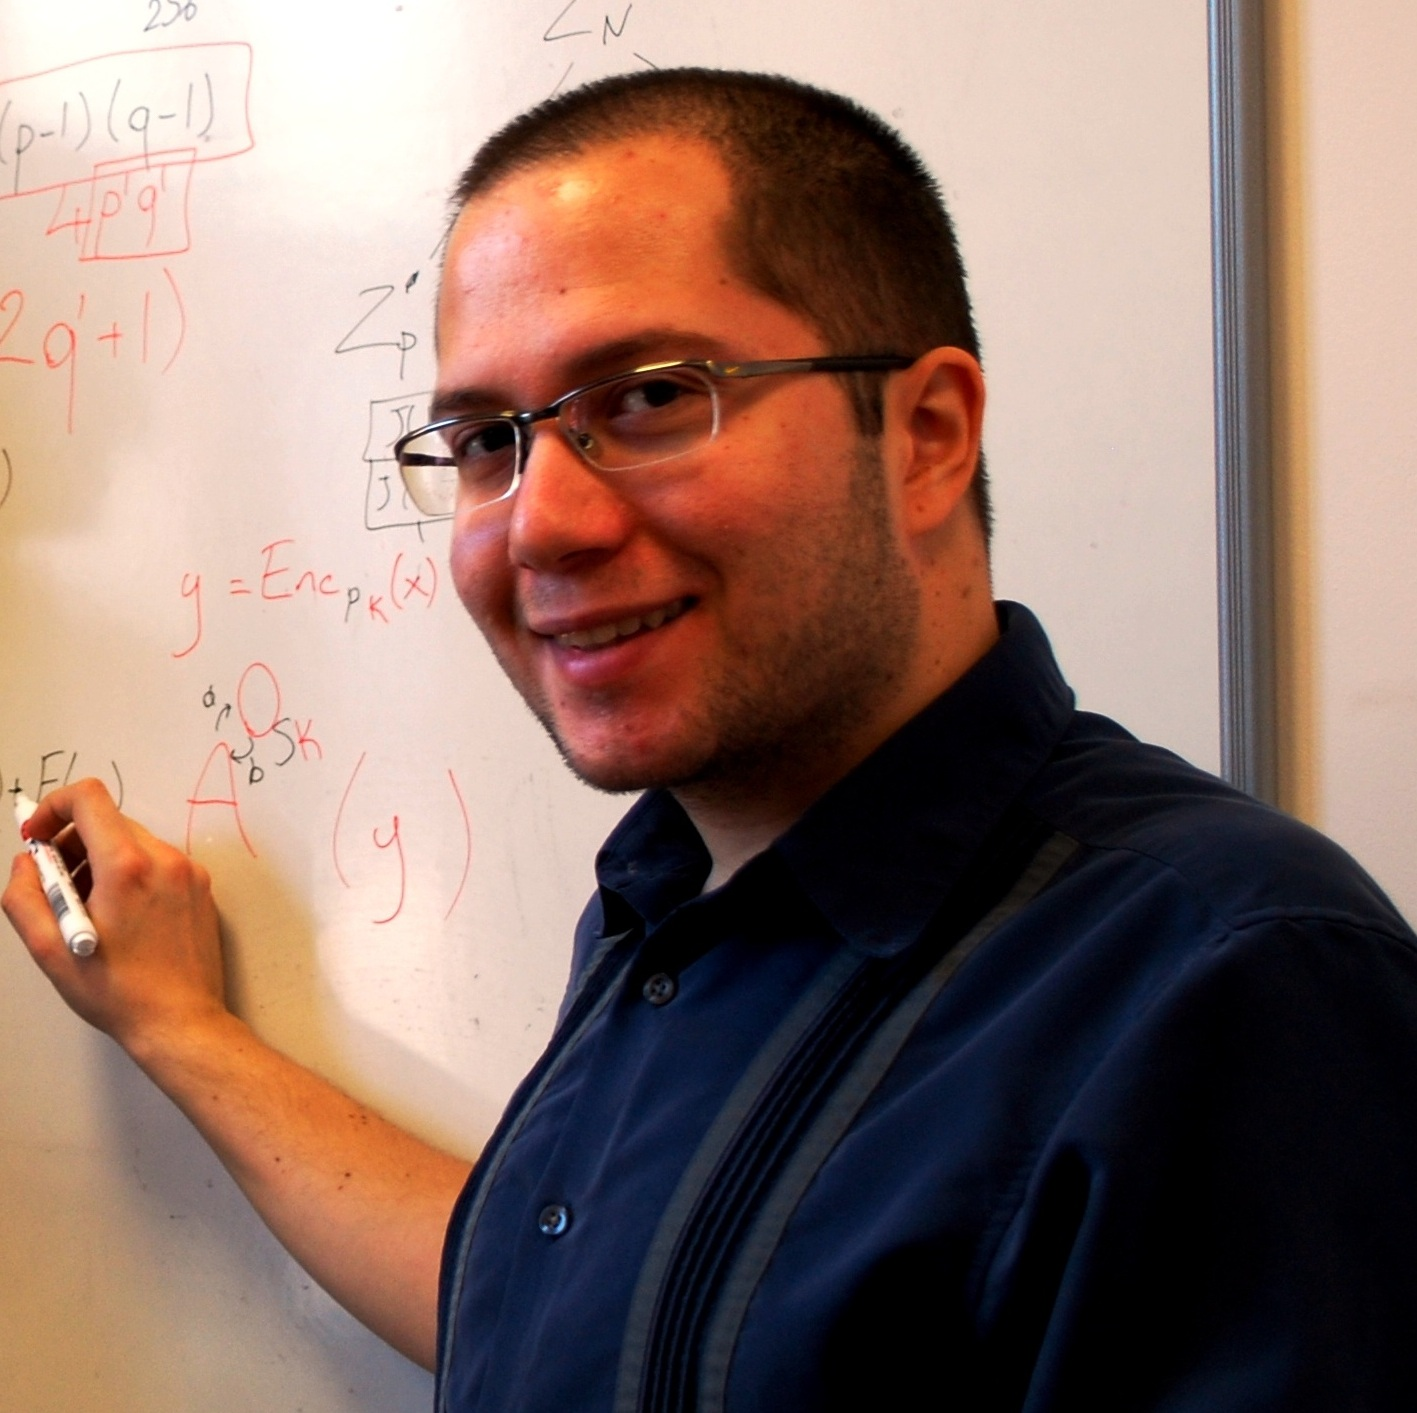
\includegraphics[width=1in,height=1.25in,clip,keepaspectratio]{authors/alptekinkupcu3.jpg}}]
{Prof. ALPTEKİN KÜPÇÜ}~received his Ph.D. degree from Brown University Computer Science Department in 2010. Since then, he has been working as a faculty member at Koç University, leading the Cryptography, Cyber Security \& Privacy Research Group that he founded. He is an ACM and IEEE Senior Member, and a co-founder of Xtinge Technology Inc.
\end{IEEEbiography}
\fi
